\section{Ceny bytů napříč roky - rozděleny podle typu}

\begin{lstlisting}[
           language=SQL,
           showspaces=false,
           basicstyle=\ttfamily,
           commentstyle=\color{gray},
           keywordstyle=\color{cyan}
        ]
SELECT 
    toYear(Time_Dimension.year) as Rok, 
    avgIf(resale_price, flat_type = '1 ROOM') as `1-room`, 
    avgIf(resale_price, flat_type = '2 ROOM') as `2-room`, 
    avgIf(resale_price, flat_type = '3 ROOM') as `3-room`, 
    avgIf(resale_price, flat_type = '4 ROOM') as `4-room`, 
    avgIf(resale_price, flat_type = '5 ROOM') as `5-room`, 
    avgIf(resale_price, flat_type = 'MULTI-GENERATION') 
        as `Multi-generation`, 
    avgIf(resale_price, flat_type = 'EXECUTIVE') 
        as `executive` 
FROM 
    FactTable 
JOIN 
    Property_Dimension ON 
        Property_Dimension.Index = FactTable.PropertyKey 
JOIN 
    Time_Dimension ON 
        Time_Dimension.Index = FactTable.TimeKey 
GROUP BY 
    Rok;
\end{lstlisting}

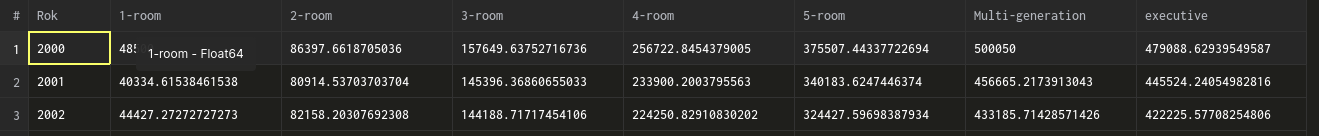
\includegraphics[width=150mm]{priceperyear-data.png}

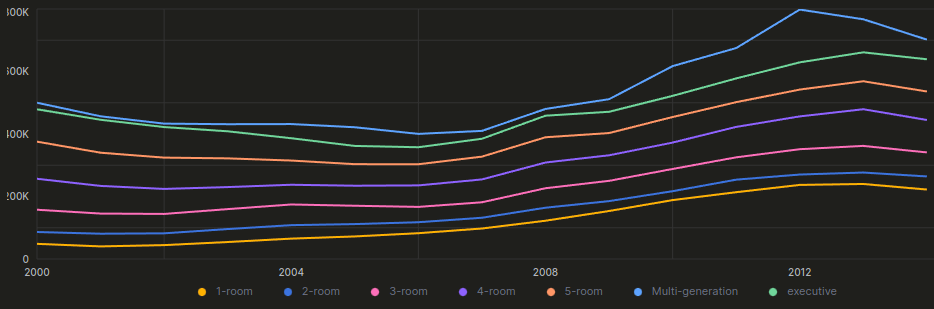
\includegraphics[width=150mm]{priceperyear.png}

